\documentclass[runningheads,a4paper]{llncs}

\usepackage[latin1]{inputenc}
\usepackage{amssymb}
\usepackage{amsmath}
\setcounter{tocdepth}{3}
\usepackage{graphicx}
\usepackage{multirow}
\usepackage{rotating}
\usepackage{url}
\usepackage{caption}
\usepackage{subcaption}
\captionsetup{compatibility=false}

\newcommand{\keywords}[1]{\par\addvspace\baselineskip
	\noindent\keywordname\enspace\ignorespaces#1}
\captionsetup[table]{skip=10pt}
\setlength{\belowcaptionskip}{-10pt}

\providecommand{\tabularnewline}{\\}

\begin{document}
	
	\mainmatter
	
	\title{The story of their lives: Massive procedural generation of heroes' journeys using evolved agent-based models and logical reasoning}
	
	
	\titlerunning{The story of their lives}
	
	\author{Rub\'en H. Garc\'ia-Ortega\inst{1} \and Pablo Garc\'ia-S\'anchez\inst{1} \and Juan J. Merelo\inst{1} \and Ar\'anzazu San-Gin\'es\inst{2} \and \'Angel Fern\'andez-Cabezas}
	%\author{Mustrum Ridcully\inst{1}}
	%
	\authorrunning{Rub\'en. H. Garc\'ia-Ortega et al.}
	%\authorrunning{R. H. P. Garc\'ia-Ortega et al.}
	% (feature abused for this document to repeat the title also on left hand pages)
	
	% the affiliations are given next; don't give your e-mail address
	% unless you accept that it will be published
	\institute
	{
		Dept. of Computer Architecture and Technology,
		University of Granada, Spain
		\and Dept. of Philosophy I, University of Granada, Spain
	}
	
	%\institute{Unseen University of Ankh-Morpork}
	
	%
	% NB: a more complex sample for affiliations and the mapping to the
	% corresponding authors can be found in the file "llncs.dem"
	% (search for the string "\mainmatter" where a contribution starts).
	% "llncs.dem" accompanies the document class "llncs.cls".
	%
	
	\maketitle
	
	%
	%%%%%%%%%%%%%%%%%%%%%%%%%%%%%%%   ABSTRACT   %%%%%%%%%%%%%%%%%%%%%%%%%%%%%%%
	%
	\begin{abstract}
		The procedural generation of massive subplots and backstories in
		secondary characters that inhabit Open World videogames usually lead
		to stereotyped characters that act as a mere backdrop for the virtual
		world; however, many game designers claim that the stories can be very
		relevant for the player's experience.
		For this reason we are looking
		for
		a methodology that improves the variability of the characters'
		personality while enhancing the quality of their backstories following
		artistic or literary guidelines. 
		In previous works,
		we used multi agent systems in order to obtain stochastic, but
		regulated, inter-relations that became backstories; later, we have used
		genetic algorithms to promote the appearance of high level behaviors
		inside them. 
		Our current work continues the previous research line and propose a
		three layered system (Evolutionary computation - Agent-Based Model -
		Logical Reasoner) that is applied to the promotion of the monomyth,
		commonly known as the hero's journey, a social pattern that constantly
		appears in literature, films, and videogames.  
		As far as we know, there is no previous attempt to model the monomyth
		as a logical theory, and no attempt to use the sub-solutions for
		narrating purposes. Moreover, this paper shows for the first time this
		multi-paradigm three-layered methodology to generate massive
		backstories.  
		Different metrics have been tested in the experimental phase, from
		those that sum all the monomyth-related tropes to those that promote
		distribution of archetypes in the characters.  
		Results confirm that the system can make the monomyth emerge and that
		the metric has to take into account facilitator predicates in order to
		guide the evolutionary process. 
		
		\keywords{Procedural generation, monomyth, agent-based model, emergent behavior}
	\end{abstract}
	
	%
	%%%%%%%%%%%%%%%%%%%%%%%%%%%%%%%   INTRODUCTION   %%%%%%%%%%%%%%%%%%%%%%%%%%%%%%%
	%
	\section{Introduction}
	\label{sec:intro}
	
	Non-player characters (NPC for further references) usually interact with the main player in order to challenge them, offer information to complete their goals or provide life-likeness to a virtual world. Following Szymanezyk et al. in \cite{szymanezyk2011individual}, crowds of NPCs enhance the game-play experience of open-world videogames. This kind of games are objective-oriented and open-landscaped videogames, following the classification by \cite{aarseth2005hunt}, where a player can explore freely a virtual world. 
	
	Open worlds are usually created using Procedural Content Generation (PGC) techniques. Recently, PCG is boosting its popularity, mainly due to two reasons: the cost reduction that the automatic generation implies to the developers, and the re-playability that it offers to the players. As a recent example, \textit{No man's sky}, an indie adventure videogame where planets, fauna and flora are created procedurally, won three Game Critics Awards, including Best Original Game and the Special Commendation for Innovation, in the past Electronic Entertainment Expo 2014, a reference annual trade show for the video game industry\footnote{\url{http://www.gamecriticsawards.com/winners.html}}.
	
	Szymanezyk et al. in \cite{szymanezyk2011individual} remark that virtual humans composing a crowd are often modeled only in terms of individuals and that research in crowd behavior identifies that a large majority of persons in real crowds do not act in individualistic terms. Characters need to explore a social network in order to augment their believability and, as simulated crowds, need to consider group aspects, hence they propose to create a network-type data structure with the help of on-going sociological work.
	The different inter-relations between the NPCs generate events and the goal of our research is to use those events to generate quality backstories for the NPCs, that are an important part of the game narrative, as defined by Bateman et al. in \cite{bateman2007game}:
	
	Backstories are the stories leading up to the events of the game, and they give the player the information they need to immerse themselves in the fiction. Since backstories are relevant for the immersion of the game, in this research, we create them massively using social interactions between the NPCs.
	
	Archetypes are recurring thematic and linguistic patterns in folklore and literature \cite{garry2005archetypes}. In videogames, archetypes are classically related to the nature of the characters (for example, thief, warrior or wizard), which reminds of the concept of stereotype, the unfair belief that all people or things with a particular characteristic are the same. An archetype is a role that a character plays in a given moment or period, regardless of the nature of their characteristics. A character could play many different archetypes in its life, even at the same time. But, what could be the minimum set of archetypes to design if we want to create interesting backstories? We found a good answer in the monomyth.
	
	The monomyth, commonly known as the hero's journey, is a pattern where
	different archetypes behave in a specific way and conform to ancient
	and modern myths from cultures all over the world: it is the story of 
	someone who is considered a hero, that has to deal with his/her
	shadow, who is waiting at the end of a journey, where different
	characters appear like mentors, allies or obstacles. The monomyth was
	studied by Joseph Campbell in `The Hero with a Thousand
	Faces'~\cite{campbell2008hero}, and later by Vogler in `The writer's
	journey'~\cite{vogler2007writer}. The monomyth has been typically
	applied to literature and traditional media, but it actually manifests
	also in modern videogames like Mass Effect or Skyrim
	\cite{knopf2013rationalist} among others. In videogames, the
	\textit{monomyth} is used to design the main plots that the player can
	empathize with: in his work \cite{bartle2004massively}, Bartle
	identifies and examines the application of key elements of the
	monomyth to videogames, and discovers that players play virtual worlds
	as a mean for self-discovery, by subconsciously, following a
	predetermined path: the monomyth. Our work uses the monomyth as a
	frame for backstories in videogames, since it provides a basic but
	omnipresent set of high level behaviors that can be found in the daily
	life but also in the biggest adventures. We use the monomyth as metric
	of interest in order to promote the archetypes present in it. 
	
	Our research uses a virtual world inhabited by autonomous agents, but
	the idea of using Agent-Based Models (ABM) of the world to generate
	stories is not new, as remarked in previous works \cite{garcia2014my}
	\cite{garciaortega2015how}, especially in the area of the interactive
	drama.
	In 2002, the Virtual Storyteller \cite{theune2002virtual} used agents
	that made up dialog using techniques from improv theater, a plot
	guide and a narrator. Our technique uses the same approach, but there
	is no plot guide. Instead, a Genetic Algorithm (GA) sets the
	mood of the backstories created by finding `archetypes'.  
	Mei et al. created in 2005 a system called Thespian \cite{si2005thespian}, where the agents' personalities, their goals, are fitted so that they are motivated to perform according to the scripts. They use look-ahead search in a decision-theoretic framework to determine the best way to achieve their goals and they are prepared to respond to the user interaction in a consistent way. Like Thespian, our work is also focused in the final script, not in modeling the agent's personality, but in our target application, open-world videogames, scripts are auto-generated in order to be re-playable.
	In 2008, Peinado et al. studied in \cite{peinado2008revisiting} the
	Belief-Desire-Intention (BDI), a cognitive model that reinforces
	narrative causality insofar as motivations and where beliefs are
	causal links that enrich characters. BDI is a theory that is starting
	to be considered a promising tool for modeling sophisticated
	characters, but it is not suitable for our research since we need to
	use more basic agents, easy to model and parametrize: as discussed by
	Sanchez and Lucas in \cite{sanchez2002exploring}, the analysis of
	relatively simple simulations using ABMs can, nonetheless, be quite
	complex, and in our case we use them in massively inhabited virtual
	worlds hard to analyze and evolve. 
	
	In previous works we used Finite State Machines (FSMs) to model the
	agent behavior, but FSMs and its variants have limitations in
	developing game Artificial Intelligence (AI). For this reason in our
	present research we have used Behavior Trees (BT) instead, following
	Lim's arguments in \cite{lim2009ai}: BTs simplify the design of
	behavior by allowing the re-usability of tasks without increasing the
	complexity of the nodes and transitions. Moreover, BTs are the most
	successful method to model AIs in videogames, and many game engines
	allow the possibility to create them, like Unity3D or Unreal Engine. A
	behavior tree consists of different kinds of tasks that are the nodes
	in a hierarchical structure, following the description by Trembley
	\cite{tremblay2012understanding}: conditions, that check properties of
	the environment, actions, that alter the state of the environment,
	and compositions, whose result is calculated from the children tasks. 
	
	Our previous work proved that a hybrid
	\textit{Evolutionary Computation - Agent Based Model} (EC-ABM)
	methodology can be used to achieve the emergence of archetypes,
	according to the structure studied by Cioffi et al. in
	\cite{cioffi2012evolutionary}. Here we add a new
	layer in charge of evaluating the backstories: the Logical
	Reasoning (LR). We use an ABM for the execution of the virtual world,
	whose execution is parametrised by a set of integer and float values,
	a Logical Reasoner that evaluates the events generated by each
	simulation and a Genetic Algorithm (GA) to find the set of parameters
	with highest fitness. The LR uses a mixed imperative-declarative
	paradigm, following Denti's approach in \cite{denti2001tuprolog}  to
	make high level deductions from the simulation's events, that are also
	expressed as logical predicates, using a logical theory that is
	modeled from the monomyth. The three layered architecture proposed can
	be observed in Figure~\ref{fig:3_layered}. 
	
	
	%
	%%%%%%%%%%%%%%%%%%%%%%%%%%%%%%  METHODOLOGY  %%%%%%%%%%%%%%%%%%%%%%%%%%%%%
	%
	\section{A backstory generator that promotes the monomyth}
	
	In this section we will present a system that uses the three-layered
	system EC-ABM-LR to generate and evaluate backstories in the virtual
	world. Firstly, Subsection \ref{sec:architecture} will present the high
	level architecture of the system and the tasks assigned to each
	logical module. Later, in Subsection \ref{sec:abm} we give the details of
	the ABM layer including the virtual world, the agent's model, the
	parametrisation of the simulation and the output format. Then, in
	Subsection \ref{sec:lr}, we propose an implementation of the logical
	model of the monomyth, and a method to evaluate the quality of the
	backstories using logical reasoning on that model. Finally, in Section
	\ref{sec:ec}, we argue the usage of a GA to promote the emergence of
	the monomyth. 
	
	\subsection{The system architecture}
	\label{sec:architecture}
	
	\begin{figure}[t]
		\centering
		\begin{subfigure}[b]{0.33\textwidth}
			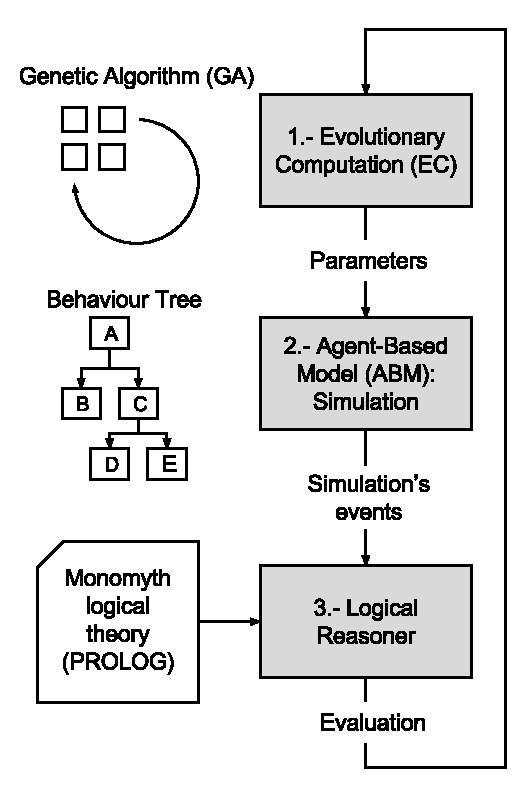
\includegraphics[width=\textwidth]{figures/3_layers.pdf}
			\caption{Proposed three-layered architecture (EC-ABM-LR).}
			\label{fig:3_layered}
		\end{subfigure}
		~
		\begin{subfigure}[b]{0.63\textwidth}
			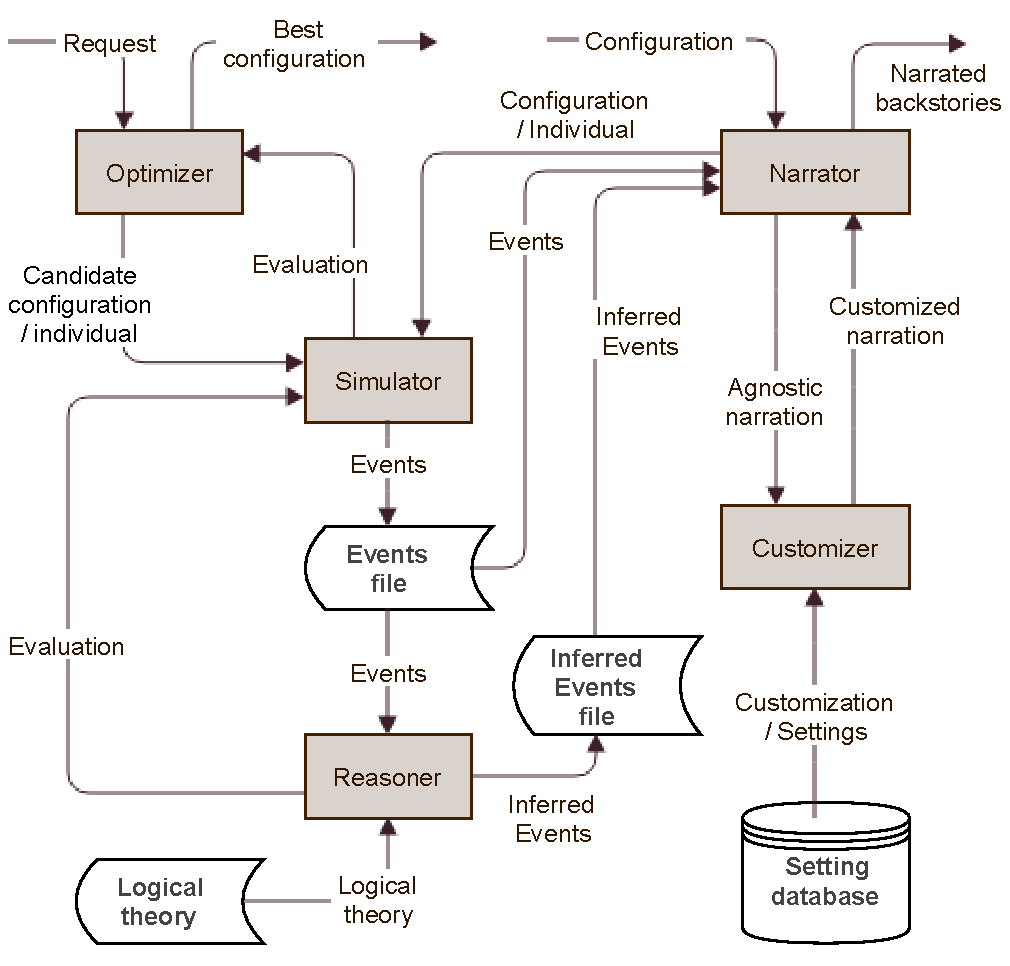
\includegraphics[width=\textwidth]{figures/made_architecture.pdf}
			\caption{Proposed components and data flow diagram of the whole architecture.}
			\label{fig:dataflow}
		\end{subfigure}
		\caption{high-level architecture of the system.}
	\end{figure}
	%
	The proposed system is described in the Dataflow Diagram in Figure
	\ref{fig:dataflow}. Different modules have been defined: the
	Optimizer, the Simulator, the Reasoner, the Narrator and the
	Customizer. The Optimizer, formerly the EC layer, uses a GA whose
	individuals are simulation configurations and returns the best
	individual found. The fitness function of each individual consists in
	several simulations, performed by the Simulator, i.e. the ABM layer,
	that uses a multi-agent system in order to generate a sequence of
	events. These events are evaluated by the LR, the third layer, that
	uses predicate logic to assign a numerical value to the events
	following guidelines extracted from the monomyth. The Simulator runs
	the virtual environment with each configuration in different trials
	and returns the average (the fitness) to the Optimizer. On the other
	hand, the Narrator takes a given solution and transforms it to an
	agnostic narration, that is a selection of relevant predicates without
	final names for the narration elements. The Customizer is in charge of
	assigning names and structures to the agnostic narration in order to
	apply a specific literary setting, for example, medieval,
	futuristic, steampunk or Shakespearian. 
	
	
	\subsection{ABM Layer: an agent-based model that generates simple events}
	\label{sec:abm}
	
	The virtual environment that we propose in this work is called
	{\sf ColorForms}, and has been designed as a board-like game that focuses
	on the four independent, ontic dimensions that conform the
	ludo-narrative design space described by Aarseth in his work
	\cite{aarseth2012narrative}: world, objects, agents and events. In our
	virtual environment, pieces will compete and collaborate in order to
	reach their desired color. 
	The narrative, as Aylett studied in
	\cite{aylett1999narrative}, emerges through small interactions between
	the characters. The main elements are described as follows:  
	
	\begin{description}
		\item[{\bf World}]: Our backstories need spatio-temporal
		dimensions, namely, a place where they occur and a time that
		sequences and orders the events. In {\sf ColorForms}, we propose
		to use a very simple map: the checkerboard, that consists of
		64 squares (8x8). The time is measured in virtual days. 
		\item[{\bf Agents}]: our agents are pieces that can occupy one
		cell each. There are three shapes for the pieces (circle,
		square and triangle) and a zero-sum game relation between
		them, rock-paper-scissors alike, in order to establish a
		method to decide the winner and the loser in individual
		direct conflicts while keeping a global balance. Agents
		change along the timeline: every piece has a background
		color and a foreground color that are constantly
		modified. The background color varies randomly in a slowly
		way for every piece and represents the continuous internal
		changes in the character needs. The foreground color can be
		changed by the piece or by other pieces under certain
		circumstances and is used to improve the happiness: the
		piece is happier when the two colors are equal.  
		\item[{\bf Objects}]: we use one type of object the
		characters must compete or collaborate for: the color spot. In
		our environment, the agents can stain with the spot in order
		to become colored. The color spots  appear or disappear randomly. 
		\item[{\bf Events}]: the characters interact between them
		and the environment, although the number of actions is very
		limited: move to a free adjacent cell, push another agent to
		a  % push to a what? - JJ
		depending on the shape, interchange the background color
		and stain with a color spot. 
	\end{description}
	
	As the we remarked in the introduction and following 
	\cite{szymanezyk2011individual}, characters need to explore a social
	network in order to augment their believability. The social component
	is defined in {\sf ColorForms} by an affinity matrix: each piece has
	an affinity with every other piece in the board, that will depend on
	their shape, background and foreground colors. This affinity is
	dynamic and will influence the decisions that piece makes; for
	instance, the happiness of the piece will be influenced by the ones with
	high affinity with it. 
	
	In our proposal, events are represented as logical predicates. Formerly, Kim defined the events in his theory of the structured
	complexes~\cite{kim1976events} using the canonical notation $[x, P, t]$, where $x$ is the
	substance, $P$ is the property it exemplifies and $t$ is the time. The
	existence condition implies that $Event [x, P, t]$ exists just in case
	that substance x has the property P at the time t. In our work, the
	events that compound the backstories are defined as meaningful logical
	predicates with notation $Predicate (t, x_0, \dots , x_n)$ where t is
	the time, and each x is an element of the world (a character, a cell,
	a moment, the property of an element or a value). Each predicate has a
	name, a signature (or arguments) and an interpretation, that is a
	description of the event in natural language. We contemplate two types of predicates: those that
	have been generated by the agents in the virtual environment (world's
	facts, present in Figure~\ref{fig:predicates}) and those that are inferred using the Reasoner
	module, related to the monomyth (world's deductions, present in Figure
	\ref{fig:theory}). White nodes in the Figure represent the predicates
	that can be generated by the ABM layer, while the gray ones are inferred by the Reasoner. The light gray nodes (called {\em helpers}) help to promote
	the dark-gray predicates, or {\em facilitators}. These are the ones
	that are present in the monomyth pattern, and they are interesting by
	themselves. Therefore, the {\em monomyth} node implies the appearance
	of all the {\em facilitators}. This node represents the `pure' literary
	monomyth.
	
	The virtual environment created for this work, the pieces (characters)
	are emotion-driven and can perform different strategies to interact
	with each other in order to generate events that will conform later
	backstories. The behavior tree used, described in
	Figure~\ref{fig:bt_autogen}, has condition nodes and action nodes;
	when a condition is fulfilled it generates an event from the Figure~\ref{fig:predicates}.c and when an action is executed correctly it
	generates an event from Figure \ref{fig:predicates}.d. Our implementation
	of behavior tree executes the tree in pre-order until a leaf node is
	evaluated as 'success'.
	
	\begin{figure}[htb]
		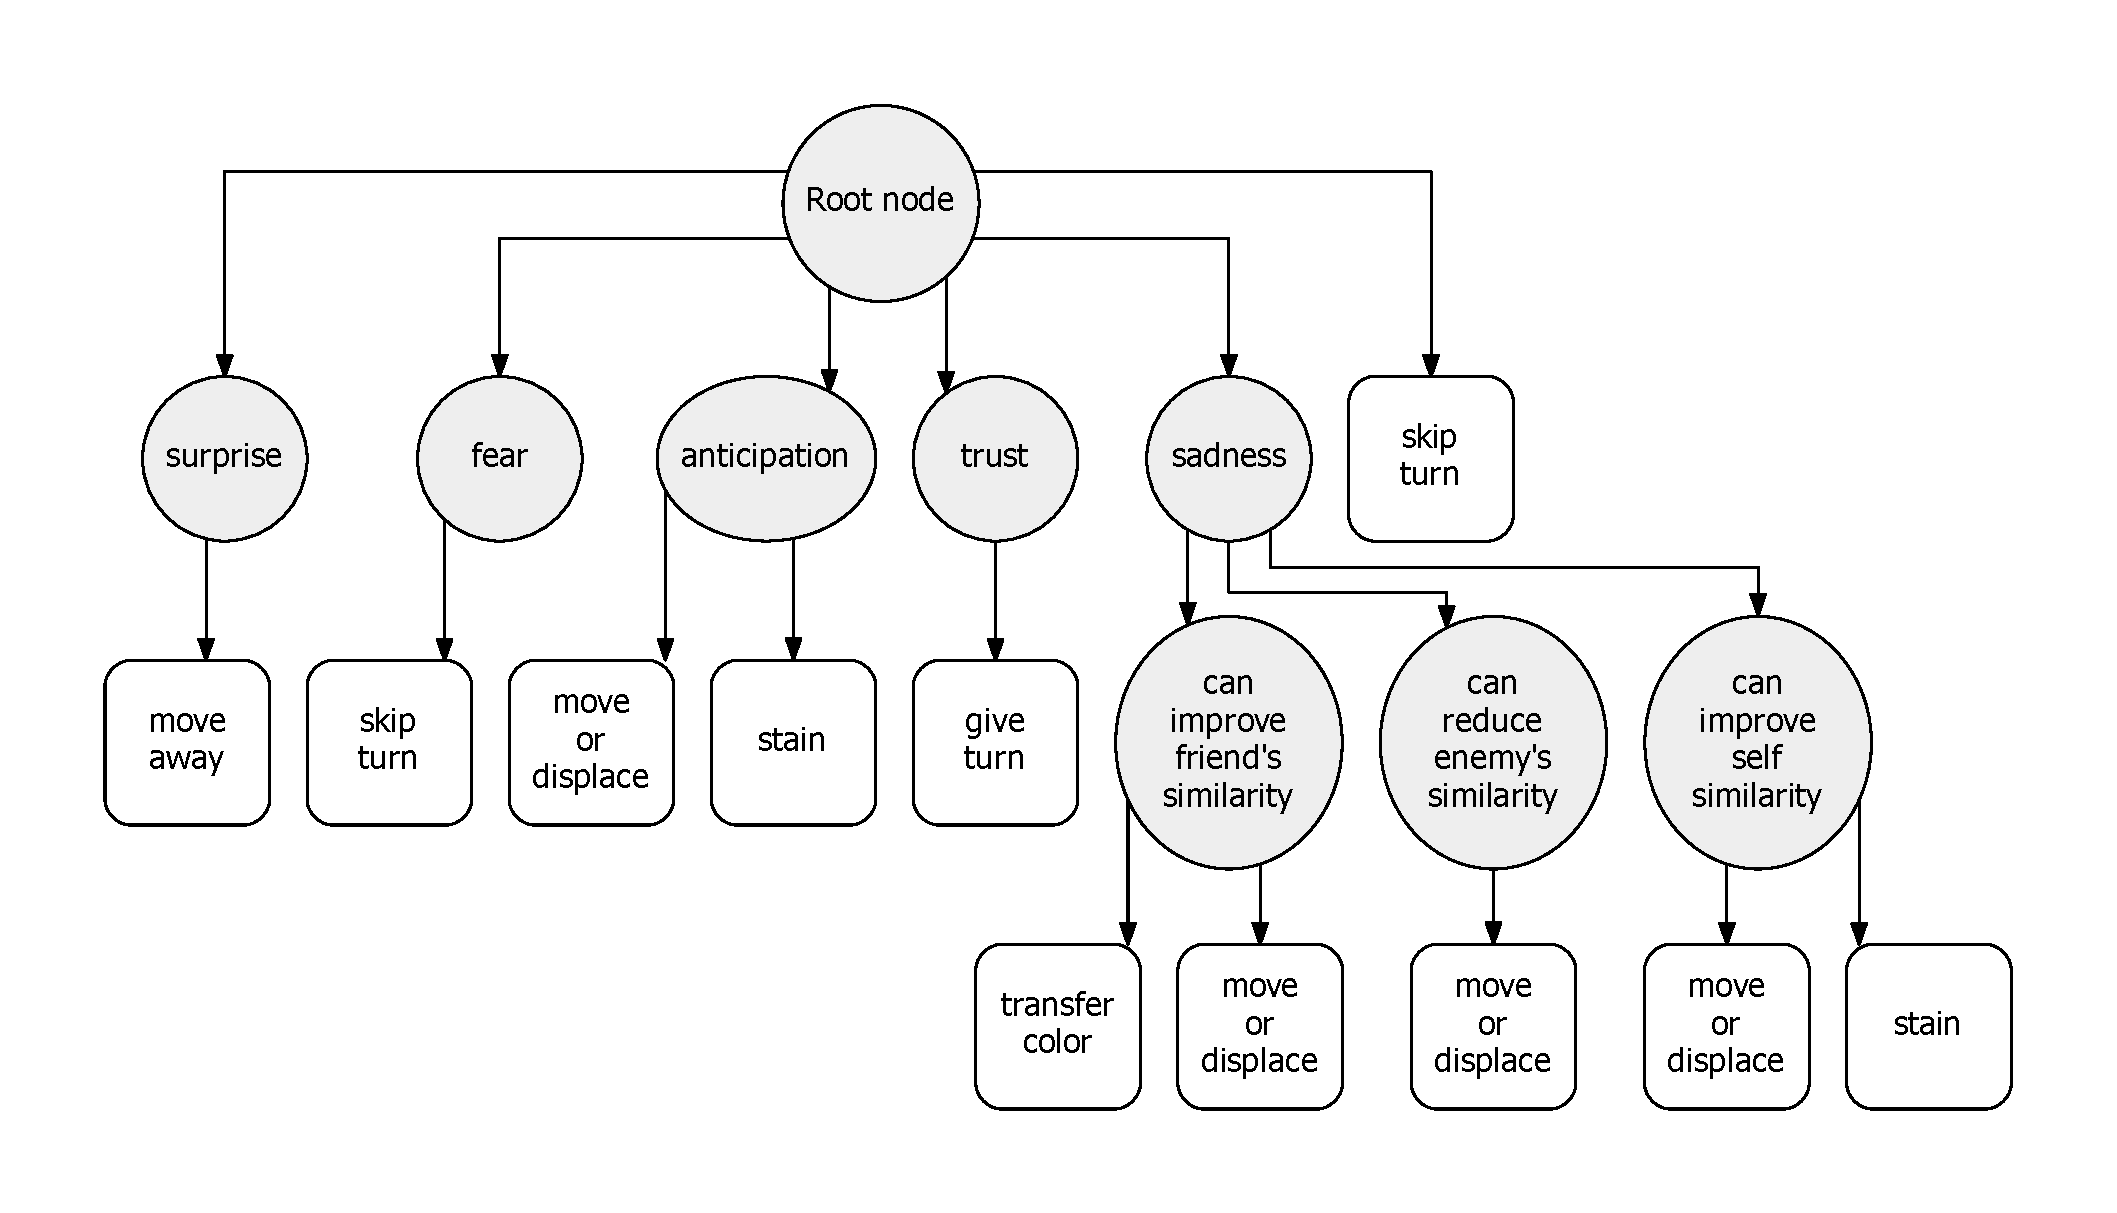
\includegraphics[width=\textwidth]{figures/bt_autogen.pdf}
		\caption{Proposed agents' behavior tree: circular nodes represent conditions and rectangular nodes represent actions.)}
		\label{fig:bt_autogen}
	\end{figure}
	
	\begin{figure}[h!tbp]
		\centering
		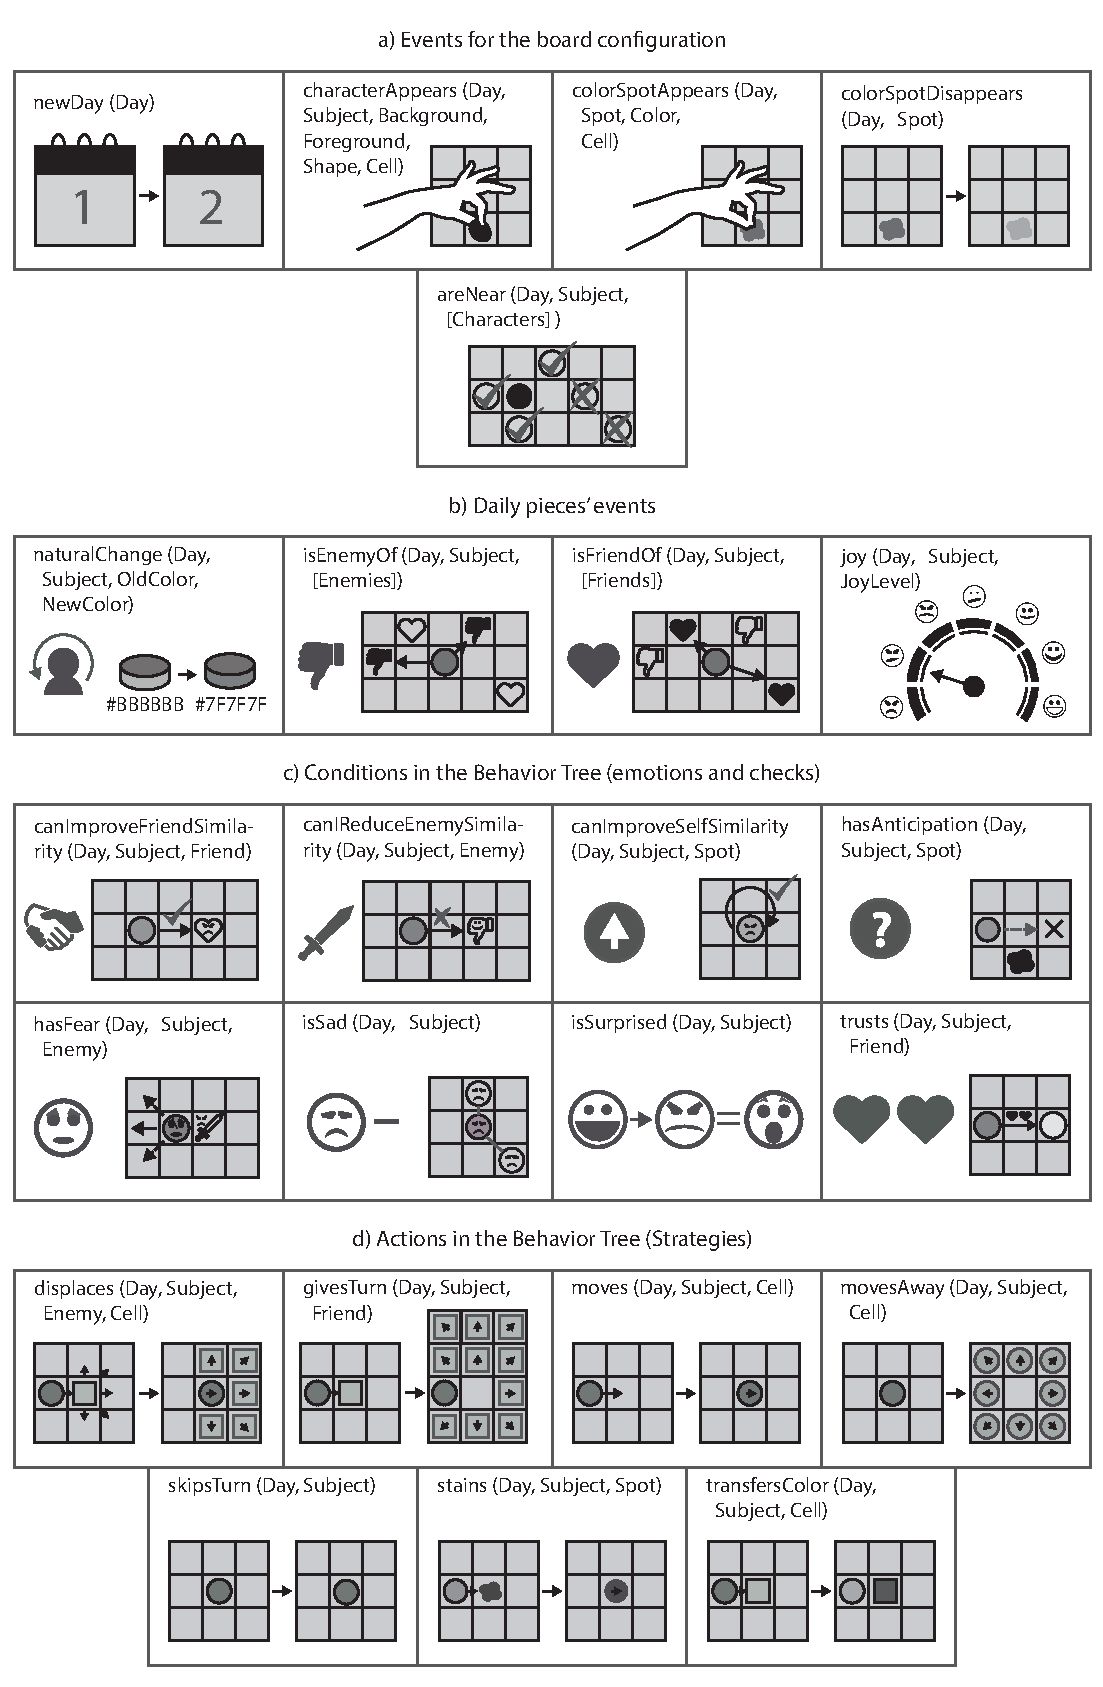
\includegraphics[width=1\textwidth]{figures/predicates.pdf}
		\caption{Predicates generated by the Simulator (world's events).} 
		\label{fig:predicates}
	\end{figure}
	
	% Use this to avoid double CR - JJ
	The Simulator takes an array of 52 values as input, maps them to the environment internal variables and performs the execution of the virtual world by running sequentially the parametrised agents' behavior tree. Finally, when a specific number of virtual days is reached, the simulation finishes and the generated events are sent to the Reasoner for further analysis. The structure of the configuration array and the meaning of each element are described in Figure~\ref{fig:abm_parameters}. As we will see in further sections, the configuration array of the Reasoner will be the chromosome in the Optimizer, in other words, the individual of the GA.
	
	
	\subsection{LR layer: logical reasoning to construct the monomyth}
	\label{sec:lr}
	
	As remarked in Section~\ref{sec:intro},
	the monomyth is a pattern that conforms the quintessence of heroism in literature and is composed of different archetypes. Vogler in \cite{vogler2007writer} encountered that archetypes are not `rigid character roles' but `flexible character functions' performed to achieve certain effects in the story, hence the same character can play different archetypes along a story.
	`There are, of course, many more archetypes; as many as there are human qualities to dramatize in stories', 
	but we will focus in the eight archetypes that conform the monomyth: the \textbf{Hero}, the \textbf{Mentor}, the \textbf{Threshold Guardians}, the \textbf{Herald}, the \textbf{Shapeshifter}, the \textbf{Shadow}, the \textbf{Ally} and the \textbf{Trickster} (see Table~\ref{tab:archetypes} for detailed definitions).
	
	\begin{table}[h!tb]
		\scriptsize
		\begin{center}
			\def\arraystretch{1.5}
			\setlength\tabcolsep{0.1cm}
			\begin{tabular}{| p{1.5cm} | p{3cm} | p{7cm} |}
				\hline
				\textbf{Trope} 
				& \textbf{Brief definition} & \textbf{Interpretation in {\sf ColorForms}} \\ \hline
				
				Conflict & (Not present in the definition of monomyth) & A sequence of events that succeed in a certain moment where two characters take part (the winner and the loser). A conflict might appear when a piece scares or displaces other, or when it takes a color spot that the other desires. If two pieces are friends and one of them is displaced by a third one, the two friends have a \textit{Conflict} with it. \\ \hline
				
				Journey & (not present in the definition of monomyth) & The time interval between \textit{Conflicts} with the same pieces. The first \textit{Conflict} must be lost by one of them (the \textbf{Hero}) and the second one has to be lost by the other (the \textbf{Shadow}), who must be `more evil' than the \textit{Hero}, that is, have helped less friends.\\ \hline
				
				Hero & The character that is willing to sacrifice his own needs on behalf of others. & The piece that loses the first conflict and wins the second one in a \textit{Conflict}.\\ \hline
				
				Mentor & The character that teaches and protects the \textit{Hero} and gives them gifts. & A piece that has high affinity with the \textit{Hero} during the \textit{Journey} and helps them at least once. \\ \hline
				
				Threshold Guardians & The  forces that the hero must overcome. & Losers of \textit{Conflicts} against the \textit{Hero} in a \textit{Journey} 
				\\ \hline
				
				Herald & The caller to the adventure for the hero. &  A piece with high affinity with the \textit{Hero} in a \textit{Journey} and that lost the first \textit{Conflict} with the \textit{Shadow}. \\ \hline
				
				Shapeshifter & The character that changes along the journey. & A piece that plays \textit{Ally} and \textit{Threshold Guardian} archetypes in the same \textit{Journey}.
				\\ \hline
				
				Shadow & The villain or antagonist; the dark side. & The character that wins the first conflict and loses the second one in a Journey. \\ \hline
				
				Ally & The character that accompanies or helps the \textit{Hero} through the \textit{Journey}. & A piece that gives the \textit{Hero} an extra turn to accomplish its goals or stays aside the \textit{Hero} in the board.\\ \hline
				
				Trickster & A mischief-maker. & A piece that stays aside the \textit{Hero} in the board and is trickier than it (joking and turning tricks, in other words, having a higher level of Joy).\\ \hline
				
			\end{tabular}
			\caption{Comparison of theoretical archetypes in the Monomyth and their interpretations in {\sf ColorForms}.}
			\label{tab:archetypes}
		\end{center}
	\end{table}
	
	In our approach, we try to define the archetypes in terms of the world's events
	described in Section~\ref{sec:abm}. The Reasoner uses a logical theory
	in PROLOG, that is a powerful approach since it gives us the
	possibility to compound predicates and use time-frameworks. The terms
	in our theory are shown in Figure~\ref{fig:theory} in an ordered way
	following a dependency graph. The monomythic archetypes are open to interpretations and can be instantiated in many different ways inside a specific story, as many as different films, books, comics or videogames with a hero we could think about. For this reason, we have implemented our own interpretation of the Monomyth archetypes in {\sf ColorForms}, that are described in the third column of Table~\ref{tab:archetypes}. 
	%
	\begin{figure}[h!tb]
		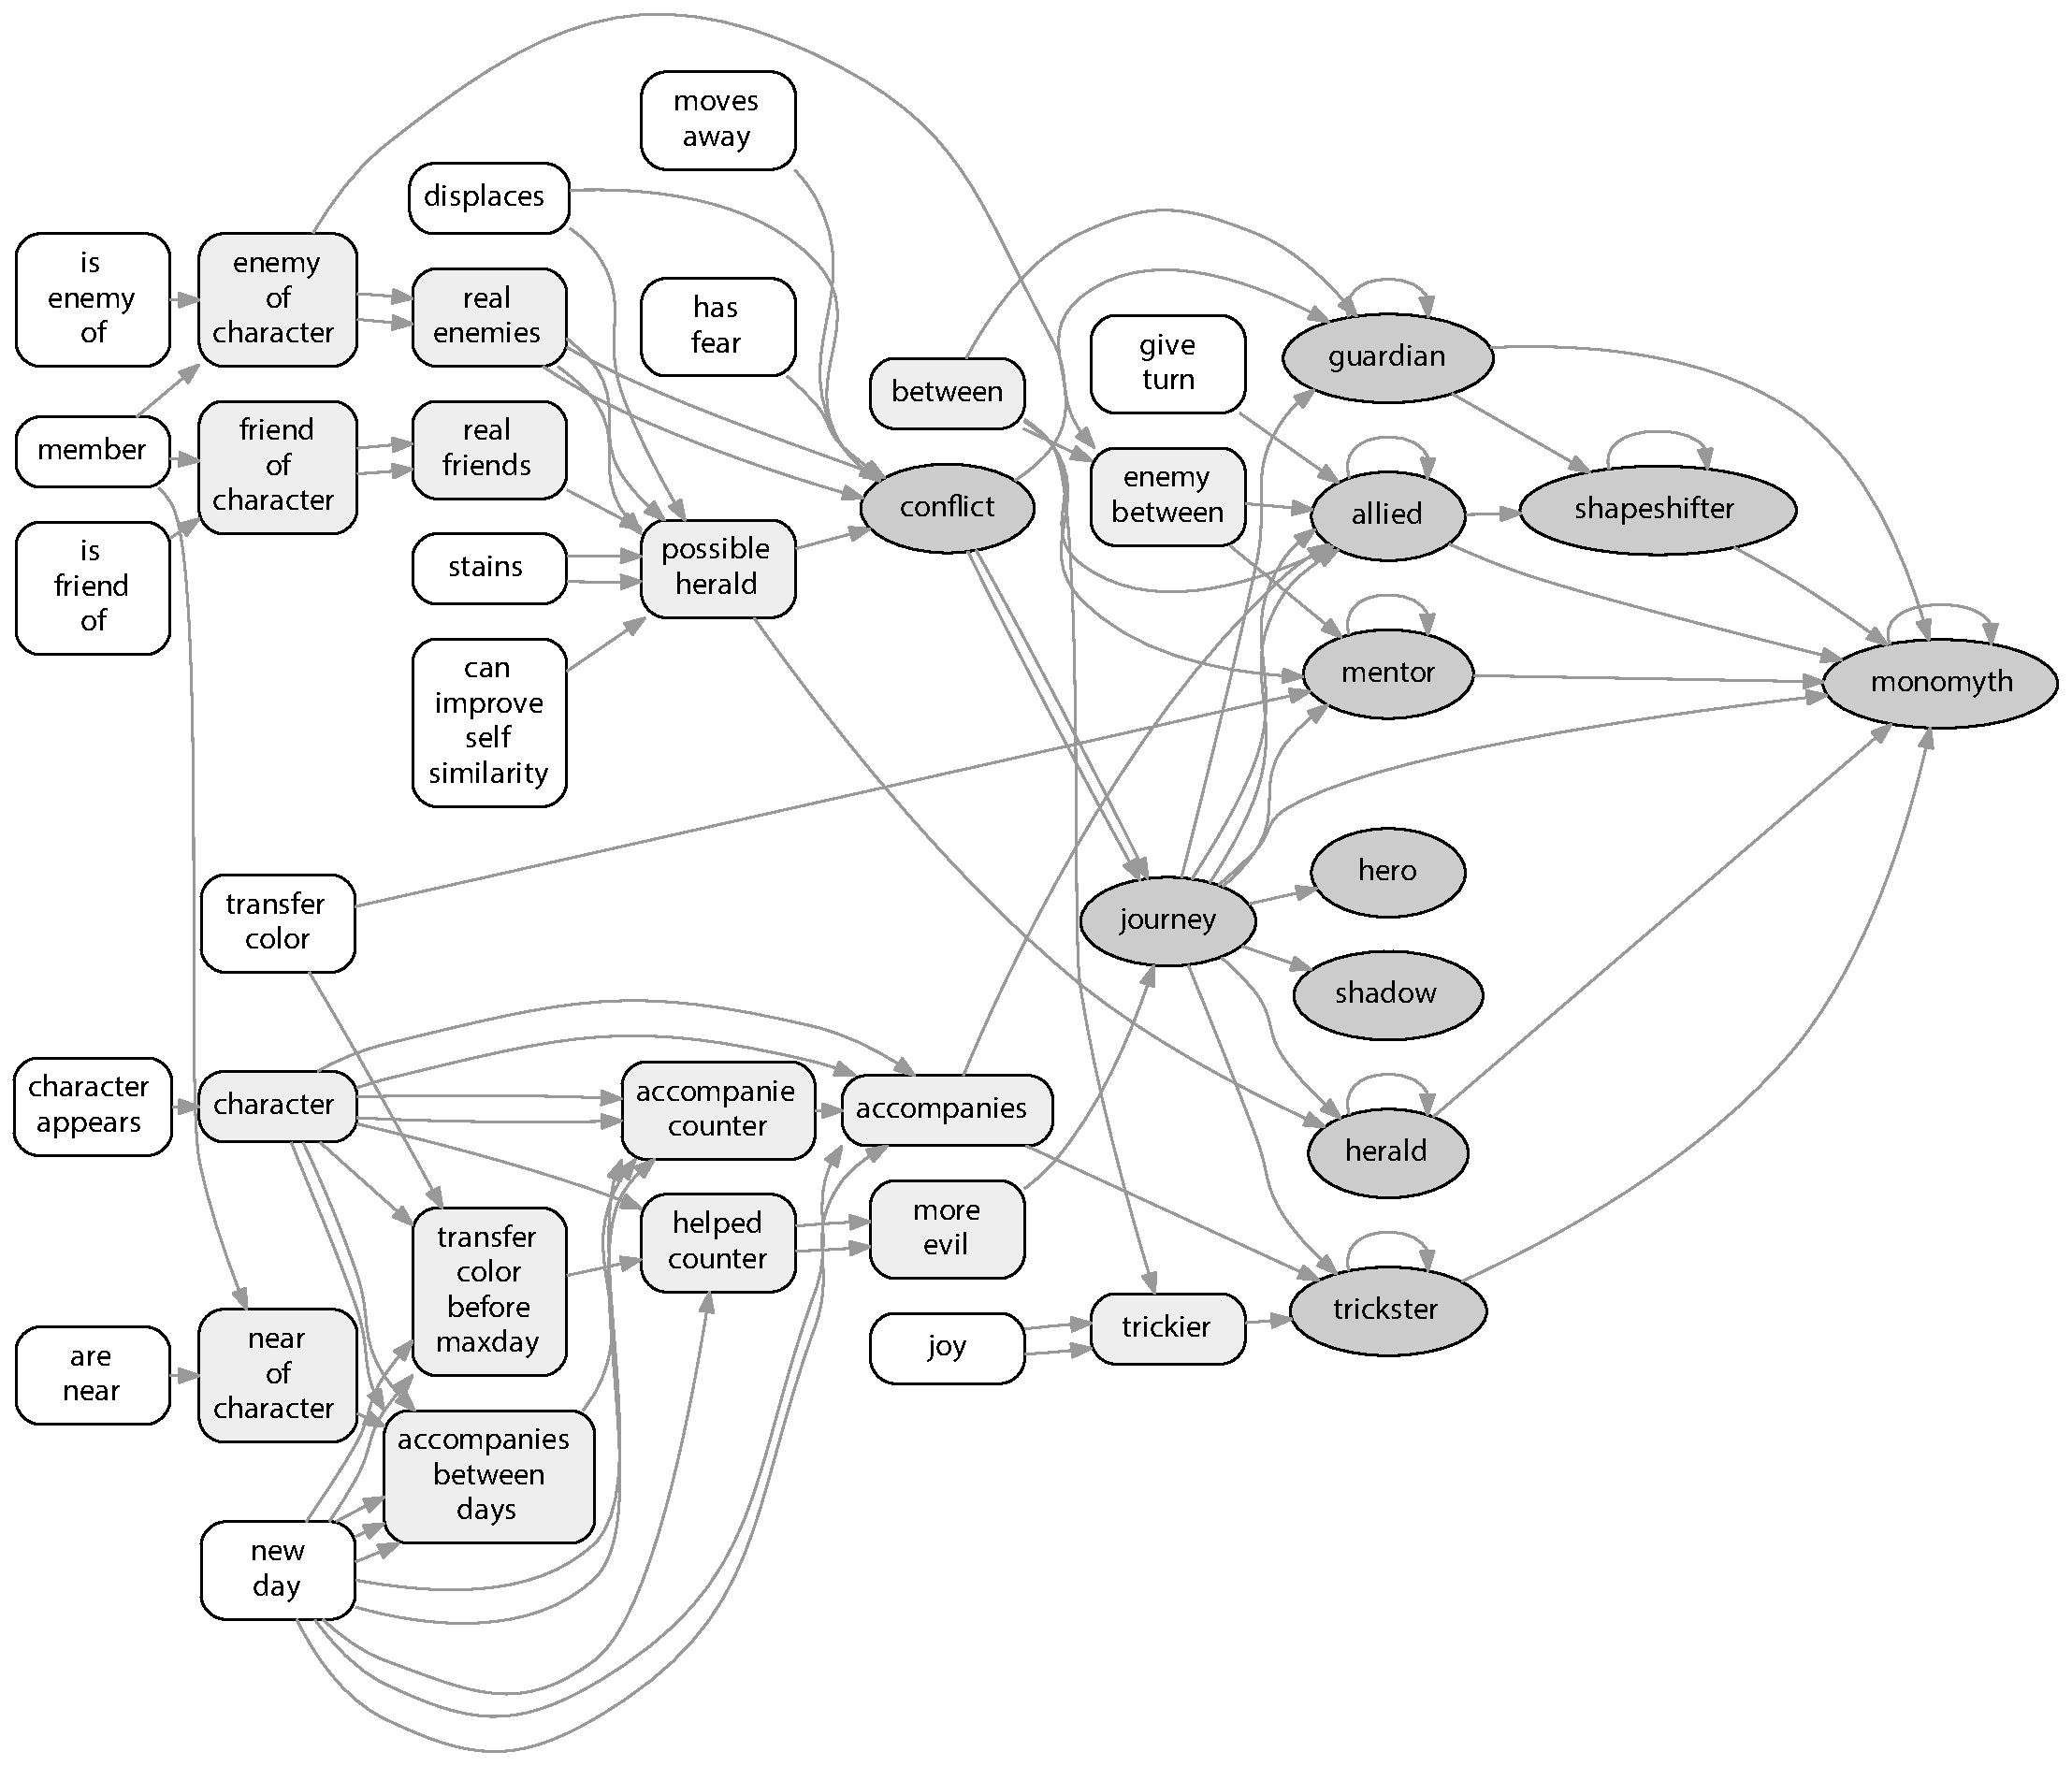
\includegraphics[width=\textwidth]{figures/theory.pdf}
		\caption{Predicate dependencies in the proposed logical theory
			of the monomyth: white nodes represent predicates that can be generated by the ABM layer and gray predicates (helpers) are inferred
			by the Reasoner. Dark-gray predicates (facilitators) conform
			the monomyth.} 
		%Algunos errores aqu�: near of -> close to
		% trickier??? 
		% joy -> happiness
		%  has fear -> fears o is afraid
		% 
		\label{fig:theory}
	\end{figure}
	
	
	
	\subsection{EC layer: genetic algorithms for the archetypes emergence}
	\label{sec:ec}
	
	The objective of our work is to generate the archetypes present in the
	monomyth. The usage of a GA is proposed, since we have to deal with a big amount of parameters. Also, because
	the result of the simulations is uncertain, due the stochastic nature of
	the virtual world and the unpredictable inter-relationships of the
	agents. This technique has been proved
	to work successfully in generative storytelling by Nairat in his
	work~\cite{nairat2011character}, and later by \cite{garcia2014my} and
	\cite{garciaortega2015how}. 
	
	\begin{figure}[ht]
		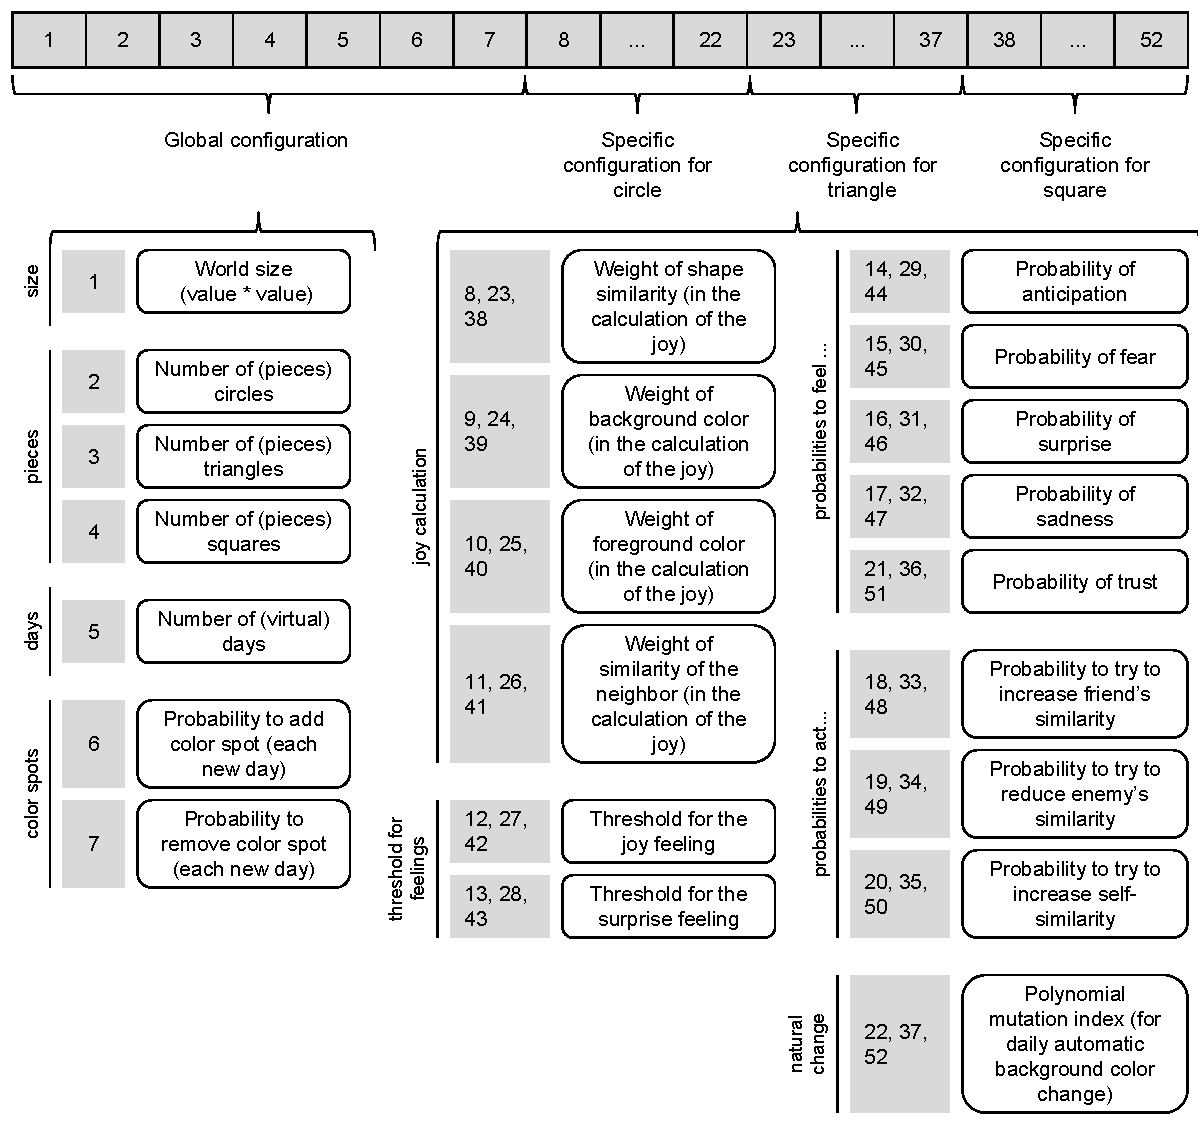
\includegraphics[width=\textwidth]{figures/abm_parameters.pdf}
		\caption{Configuration array of the Reasoner (ABM layer) and
			structure of the individual of the Optimizer (EC
			layer). Gray rectangles stand for the index of the
			parameters.} 
		\label{fig:abm_parameters}
	\end{figure}
	
	%GAs are a subset of Evolutionary Algorithms (EAs), which are a set of
	%bio-inspired techniques applied to optimization problems
	%\cite{eiben2010whatis}. 
	% we don't need this in a EA conference - JJ
	%% , based on the process of natural selection
	%% \cite{darwin1859}. In this kind of algorithms, a \textsc{population}
	%% of codified solutions (called \textsc{individuals}) is created. The
	%% most adapted individuals have more chances to be selected for
	%% reproduction, so their offspring could inherit their genetic
	%% material. The level of adaptation of each solution is measured using a
	%% \textsc{fitness} function, that usually models the problem to
	%% solve. GAs were proposed by Holland \cite{holland1975adaptation}, and
	%% also studied by Goldberg \cite{goldberg1988genetic} and Michalewicz
	%% \cite{michalewicz1996genetic}. In this kind of EA, the representation
	%% of the solution is a string of numbers, called \textsc{chromosome}
	%% (and sometimes \textsc{genome}). The individuals are selected
	%% proportionally to their fitness, and then \textsc{recombination}
	%% and/or \textsc{mutation} are applied to generate new individuals that
	%% will be introduced in the population. These algorithms have been used
	%% in different areas, such as function optimization
	%% \cite{michalewicz1996genetic}, combinatorial optimization
	%% \cite{Esparcia2009EVITA}, artificial intelligence in videogames
	%% \cite{Fernandez20111optimizing}, or generative art
	%% \cite{Garcia2013RGB}, among others.  
	%
	The Optimizer module uses a GA to evolve configurations of the
	Simulator in order to find the one with the best fitness, that is
	calculated in base of the predicates found by the Reasoner. The use of
	a GA is adequate since it is not possible to deduce the effects of the
	parameter values when the agents interact: the fitness is the result
	of high level interactions or specific sequences of them (phenotype)
	that cannot be predicted. This uncertainty is increased by the
	stochastic nature of the simulation, since different executions of the
	Simulator provide distinct results that improves the re-playability of
	the videogame. 
	
	An individual for our GA is a chromosome of 52 genes, where the first 5 are natural numbers in different ranges and the following 47 are real values in the range [0-1]. The structure of the chromosome is detailed in Figure~\ref{fig:abm_parameters}.
	
	
	
	The fitness used takes into account the number of archetypes that have been deduced by the Reasoner since we are interested in the promotion of the monomyth, as described in Section~\ref{sec:lr}.
	
	
	Let
	$A_i$ an archetype in the set of all $T$ desired predicates $A$:
	\begin{multline}
		A = \{Conflict, Journey, Shadow, Hero, Mentor, Herald, Guardian,\\
		Allied, Trickster, Shapeshifter, Monomyth\}
	\end{multline}
	and $|A_{i}|$ the number of occurrences of that predicate generated by the Reasoner at the end of the simulation, we define the next three metrics to evaluate the fitness $F$:
	
	\begin{itemize}
		\item Amount of Monomyth Occurrences Found ($M$): counts the number of occurrences of the predicate `monomyth', hence it stands for the most basic metric we can implement.
		\begin{equation}
			F_{M} = \left| A_{Monomyth}\right|
			\label{eq:M}
		\end{equation}
		
		
		\item Amount of All Occurrences Found ($A$): counts the number of occurrences of every monomyth-implication predicate in the simulation, defined as `facilitators' in Section \ref{sec:lr}, and also shown as dark-gray nodes in Figure~\ref{fig:theory}.
		\begin{equation}
			F_{A} = \sum _{i=0}^{T}\left| A_{i}\right|
			\label{eq:A}
		\end{equation}
		
		\item Amount of All Occurrences Distributed by Predicates ($AD$): counts the number of occurrences, but promotes the appearance of new archetypes. That is, the occurrence of two different predicates gets a bigger fitness than two occurrences of the same predicate. 
		\begin{equation}
			F_{AD} = \sum _{i=0}^{T} \log _{10} (\left|A_{i}\right| + 1)
			\label{eq:AD}
		\end{equation}
		
	\end{itemize}
	
	Although our goal is to make the monomyth emerge, and this can be achieved with fitness metric $M$ (equation ~\ref{eq:M}), we have added the extra metrics defined in equations \ref{eq:A} and \ref{eq:AD} to observe the effects of guiding the evolution by promoting the appearance of the facilitators.
	
	More complicated metrics could be chosen, for example, using human interaction as proposed by Takagi in \cite{Takagi2001}, but the chosen ones can be considered the simplest ones to detect the emergence of the monomyth. 
	
	
	%%%%%%%%%%%%%%%%%%%%%%%%%%  EXPERIMENTS AND RESULTS  %%%%%%%%%%%%%%%%%%%%%%%%%%
	%
	\section{Experiments and Results}
	
	% Qu� queremos hacer? demostrar que podemos hacer que surja el monomito y de paso si las m�tricas seleccionadas son adecuadas
	
	The objective of this paper is to demonstrate that it is possible to create a multi-paradigm three-layered system (AC-LR-ABM) that is able to generate massive backstories following the monomyth guidelines. As secondary objectives, we try to test if the chosen metrics are valid to allow the emergence in the evolutionary process of the GA. 
	
	% Parametrizaci�n del GA
	We use a generational model, with selection by binary tournament and
	no elitism. Our mutation operator is polynomial and our crossover
	operator is \mbox{blx-$\alpha$}, both good elections when our genes
	are coded as numerical values. All these decisions are supported by
	Eiben and Smith in their book \cite{eiben2010whatis}. The number of
	individuals in the populations is 30, the termination condition is to
	reach 40 generations and the maximum time to deduce the predicates
	from the world's events is 300 seconds. To reduce uncertainty in the
	evaluation of an individual, we use explicit averaging
	\cite{Jin2005303}, using the average of 15 trials.
	The range for the number of pieces is $[0-15]$ for each shape, hence
	the final solution can have $[0-45]$ pieces. The size of the world
	can vary from $8x8$ (64 cells) to $16x16$ (256). The range of virtual
	days for each simulation is $[2-128]$. These values have been selected empirically after
	preliminary tests, and are summarized in
	Table~\ref{tab:parameters_ga}. 
	
	\begin{table}[h!tb]
		\scriptsize
		\begin{center}
			\def\arraystretch{1.5}
			\setlength\tabcolsep{0.1cm}
			\begin{tabular}{| l | l |}
				\hline
				\textbf{Parameter}			  & \textbf{Value} \\ \hline
				\multicolumn{2}{|c|}{GA parameters} \\ \hline
				Type                  & generational                 \\ \hline 
				Population size       & 30                            \\ \hline
				Selection             & binary tournament             \\ \hline
				Mutation operator     & polynomial (theta = 20)       \\ \hline
				Crossover operator    & blx-$\alpha$ ($\alpha$ = 0.5) \\ \hline
				Termination condition & 30 generations                \\ \hline
				Fitness               & M / A / AD                    \\ \hline
				\multicolumn{2}{|c|}{Gene ranges} \\ \hline
				World size gene & 8 - 16 \\ \hline
				Number of circles & 0 - 15 \\ \hline
				Number of triangles & 0 - 15 \\ \hline
				Number of squares & 0 - 15 \\ \hline
				Number of virtual days & 2 - 128 \\ \hline
				\multicolumn{2}{|c|}{ABM parameters} \\ \hline
				Maximum reasoning time & 300 s \\ \hline
				Number of trials in fitness & 15 \\ \hline
			\end{tabular}
			\caption{Parameters of the GA used in the experiments.}
			\label{tab:parameters_ga}
		\end{center}
	\end{table}
	
	% Resultados experimentos
	
	The experiments are executed with the three fitness functions previously defined in Section~\ref{sec:ec}: amount of Monomyth Occurrences Found (M), Amount of Monomyth Occurrences Found ($M$) and Amount of All Occurrences Distributed by Predicates ($AD$). The results obtained can be seen in Table~\ref{fig:results}.
	
	The predicate monomyth depends directly and indirectly on a huge amount of predicates (world's events, helpers and facilitators, as the dependency graph in Figure~\ref{fig:theory} reflects) hence we cannot search it directly, as seen in the graphs called 'Fitness M' and 'Monomyth in fitness M'. However, if we guide the evolutionary process by taking into account also the facilitator predicates, as A and D do, we can make the whole monomyth emerge with our system.
	
	The fitness AD gets better solutions than fitness A, since we promote the appearance of new the predicates (and all of them are necessary for the monomyth). In graph 'Monomyth fitness A' we can observe that monomyth emerges punctually but the GA loses it in favor of new appearances of the \textit{Ally}, as the graph 'facilitators in fitness A' shows; nevertheless, it does not happen in AD, as shown in 'Monomyth in fitness AD', where the number of monomyths fluctuates but keep a tendency.
	
	Regarding the facilitators found, their rate of appearance is aligned with the real applications of the monomyth: \textit{Allies}, \textit{Threshold Guardians} and \textit{Tricksters} have much more occurrences than the rest. The \textit{Hero} and the \textit{Shadow} are the leading roles and they must appear only the necessary. Finally \textit{Shapeshifters},  \textit{Mentors} and \textit{Heralds} are uncommon characters that depends on predicates that are hard to satisfy. These appearance rates also confirms that our logical model for the monomyth is aligned with the one described by Vogler. However, the fitness AD promotes less difference in the number of appearances than fitness A. As we are not interested in the number of specific archetypes but in the number of monomyths found, we favor the use of AD.         
	
	
	% grafica de predicado monomito con los 3 fitness
	
	\begin{figure}[h!tb]
		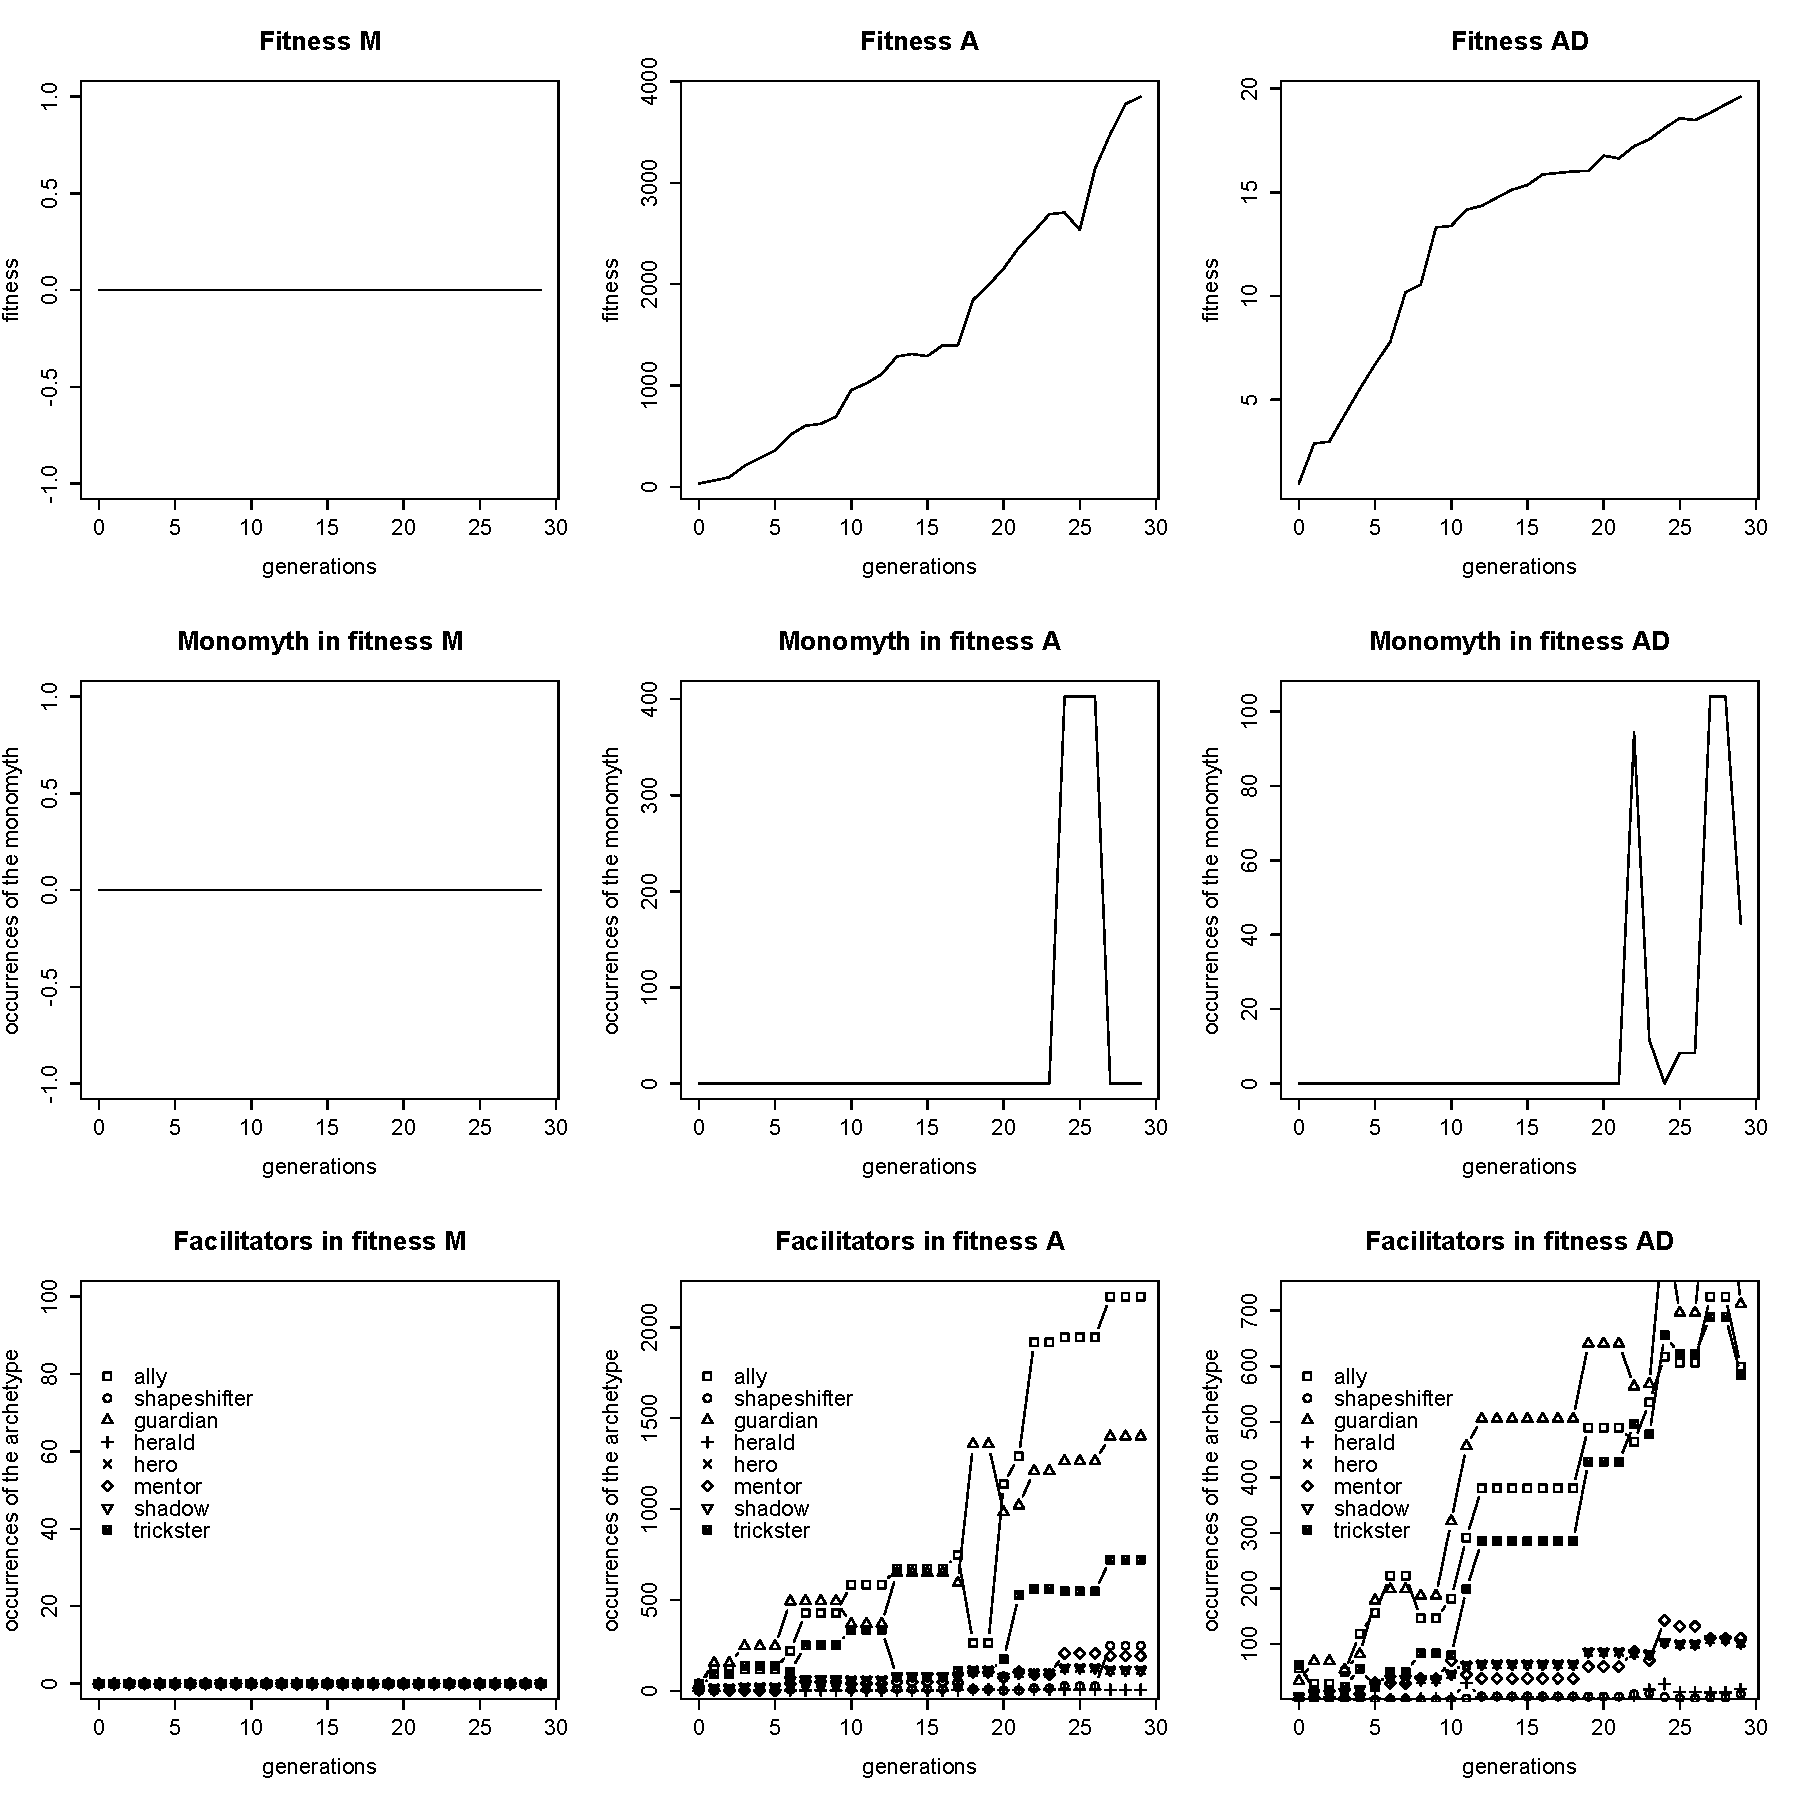
\includegraphics[width=\textwidth]{figures/results.pdf}
		\caption{Graph showing the results of running {\sf ColorForms}
			with the three different fitness
			functions; the first column belongs to M (promotion
			of the monomyth), the second column to A (promotion of the
			facilitators) and the third column to AD (promotion of the
			distribution of facilitators). The first row shows the
			evolution of the best individual, the second one the
			number of occurrences of the monomyth found and the third
			one the number of occurrences of the facilitators.} 
		\label{fig:results}
	\end{figure}
	
	% estudio de la mejor soluci�n encontrada
	
	% el c�digo fuente de los experimentos y del framework puede descargarse de ...
	
	The source code and the experiments are distributed under GPLv3
	license, and are freely available at the official project's
	page~\footnote{\url{https://github.com/raiben/made}}. 
	
	\section{Conclusions}
	
	% este trabajo presenta...
	
	The present paper uses agent-based modeling, logical reasoning and
	genetic algorithms to promote the appearance of massive backstories
	that can later be used in 
	videogames with archetypes that follow the monomyth
	guidelines. For this, we model emotion-driven autonomous agents that
	interact in a virtual world called {\sf ColorForms} where color pieces
	compete and collaborate in order to change their colors. The virtual
	environment generates events using logical predicates that are later
	used by a PROLOG reasoner to deduce the different archetypes that
	conforms the monomyth. Finally, a genetic algorithm is used to
	optimize the configuration of the virtual world. We have compared
	three different fitnesses in order to guide the evolutionary process. 
	
	% los resultados muestran que
	Experiments show that the emergence of the monomyth can be helped by
	searching facilitators, that is, the predicates that are found
	in the monomyth, instead of just focusing in the number of monomyth
	occurrences. Moreover, rewarding the diversity of archetypes usually leads to
	better solutions. Thus, these experiments prove that the
	monomyth can emerge in this kind of individual based models and it can
	be applied to massively generate backstories populated with
	archetypes; these archetypes have been  proved to be emotionally engaging for the videogame
	player. 
	
	% como trabajo futuro ...
	In future works we plan to improve the fixed Behaviour Tree structure by making it evolve using evolutionary computation, improve the narration engine and use human-guided metrics for the evolutionary process. 
	
	
	\section*{Acknowledgments}
	This work has been supported in part by projects 
	TIN2014-56494-C4-3-P and TIN2012-32039 (Spanish Ministry of Economy and Competitivity), 
	PETRA (SPIP2014-01437, funded by Direcci�n General de Tr�fico),
	PROY-PP2015-06 (Plan Propio 2015 UGR),
	PYR-2014-17 (GENIL project, awarded by CEI-BIOTIC Granada), and 
	MSTR (PRY142/14, Fundaci�n P�blica Andaluza Centro de Estudios Andaluces en la IX Convocatoria de Proyectos de Investigaci�n).
	
	
	\bibliographystyle{splncs}
	\bibliography{garcia-ortega}
	
	
\end{document}
\grid
\grid
